% !TeX root = multianalysis.tex
% !TeX encoding = UTF-8
% !TeX program = XeLaTeX


\part{聚类分析(Cluster analysis)}

\section{描述性统计}

\begin{frame}{描述性统计}
    \begin{center}
        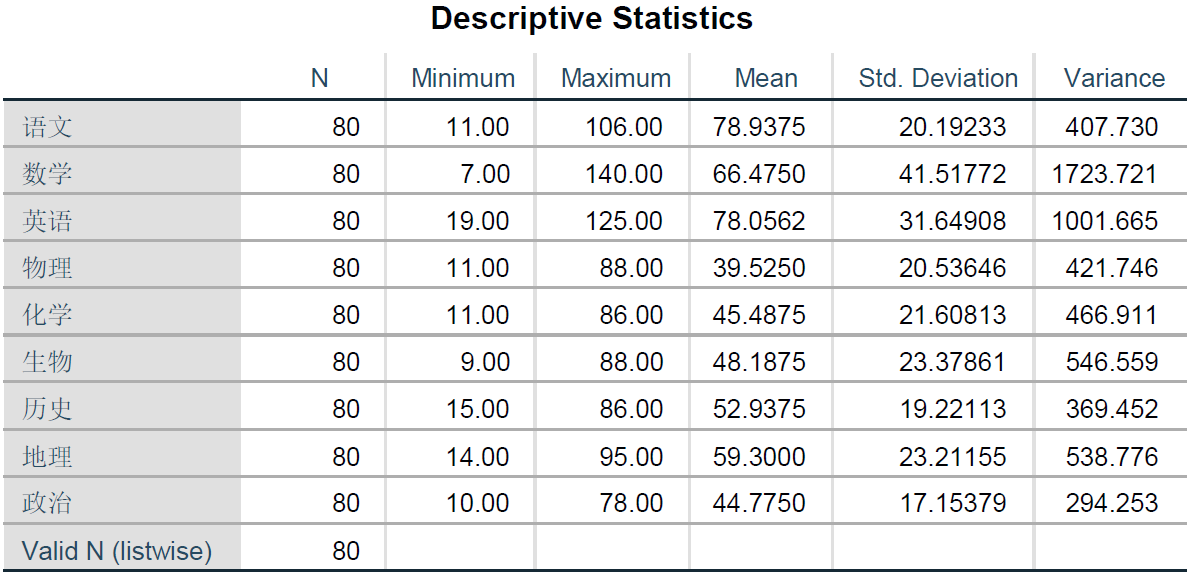
\includegraphics[scale=0.285]{descriptive.png}
    \end{center}
    \vspace{-0.5cm}
\end{frame}

\section{对指标变量(9个学科)进行系统聚类}

\begin{frame}{选择平方欧氏距离时的距离矩阵}
    \begin{center}
        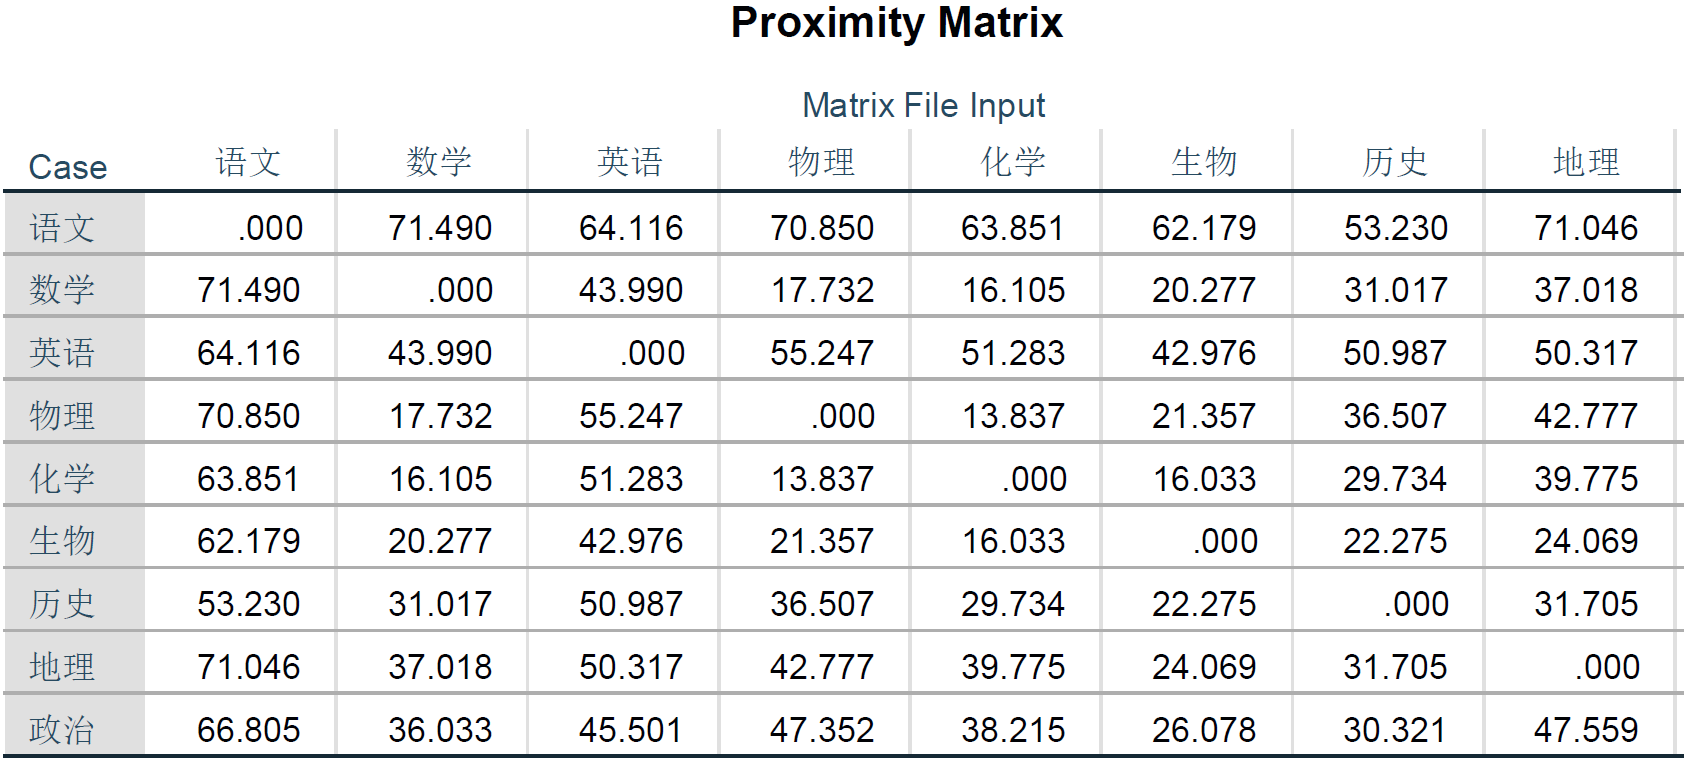
\includegraphics[scale=0.2]{平方欧氏距离距离矩阵.png}
    \end{center}
    \vspace{-0.5cm}
\end{frame}

\begin{frame}{组内联结法的谱系聚类图}
    \begin{center}
        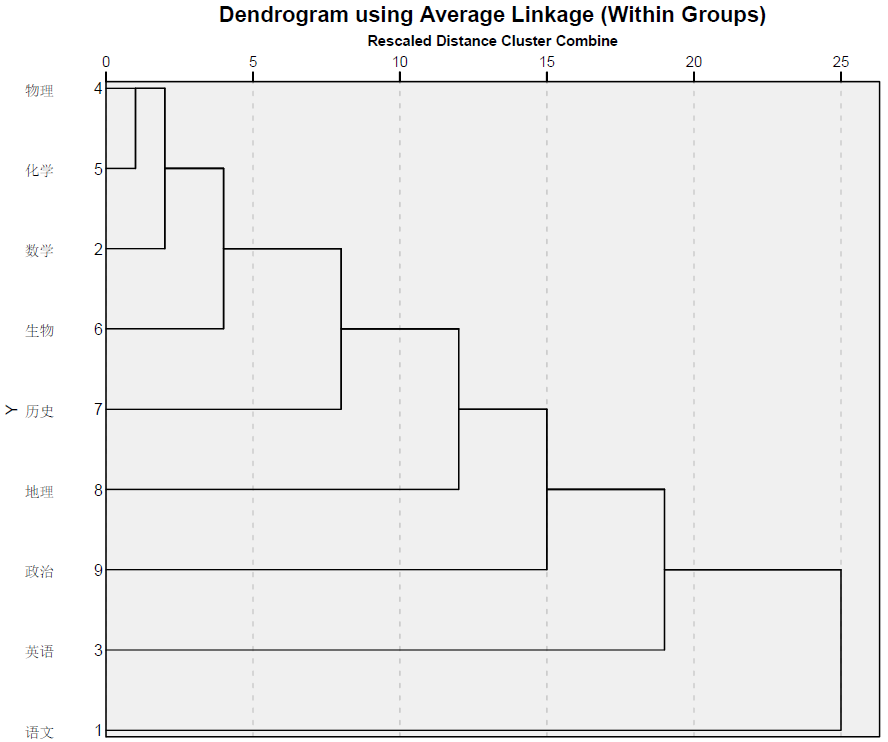
\includegraphics[scale=0.25]{组内联结法谱系聚类图.png}
    \end{center}
    \vspace{-0.5cm}
\end{frame}


\begin{frame}{选择聚成4类的结果}
    \begin{center}
        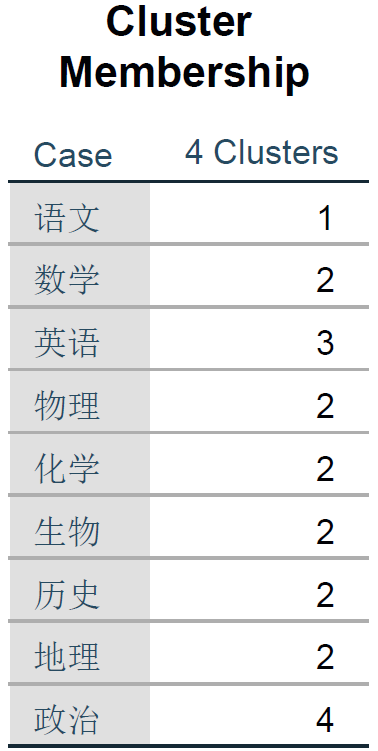
\includegraphics[scale=0.25]{聚类结果.png}
    \end{center}
    \vspace{-0.5cm}
\end{frame}


\section{对样品(80名同学)进行 K-means 聚类}

\begin{frame}{4个初始中心}
    \begin{center}
        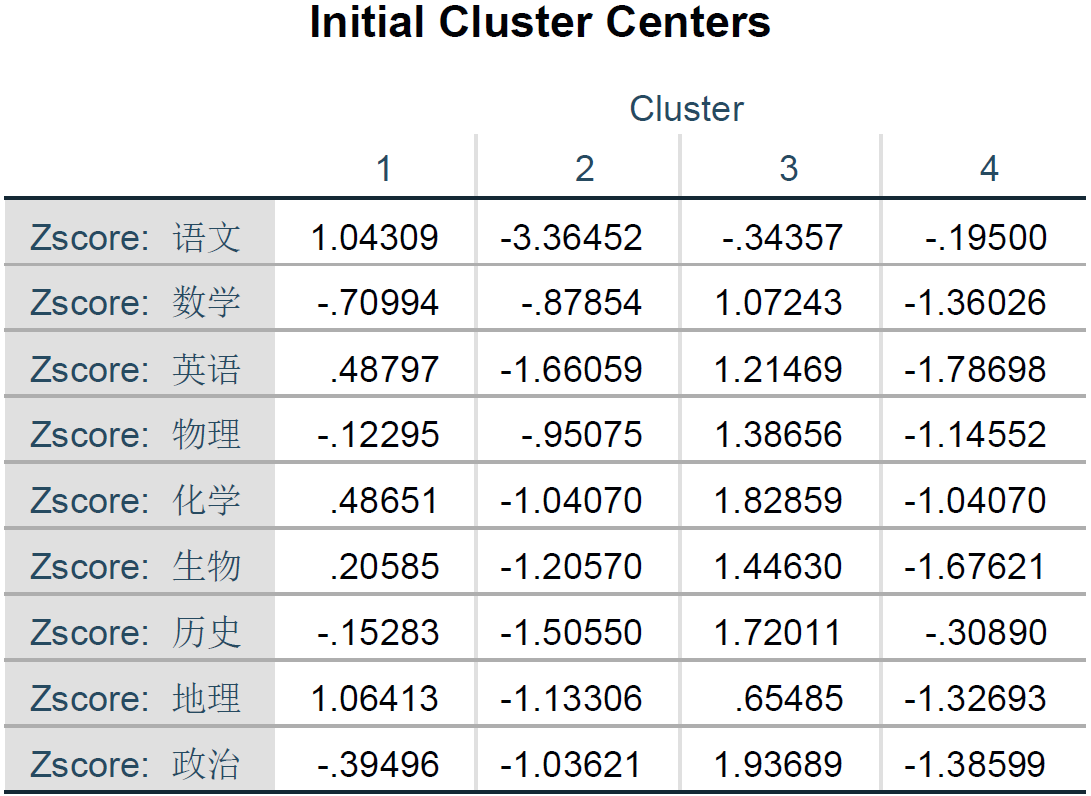
\includegraphics[scale=0.235]{4个初始中心.png}
    \end{center}
    \vspace{-0.5cm}
\end{frame}

\begin{frame}{聚类结果}
    \begin{figure}[H]
        \centering
        \begin{minipage}{0.32\textwidth}
            \centering
            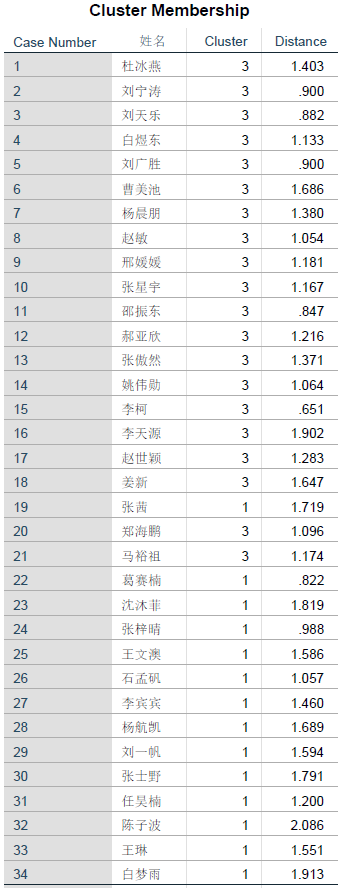
\includegraphics[scale=0.23]{聚类结果1.png}
        \end{minipage}
        \begin{minipage}{0.32\textwidth}
            \centering
            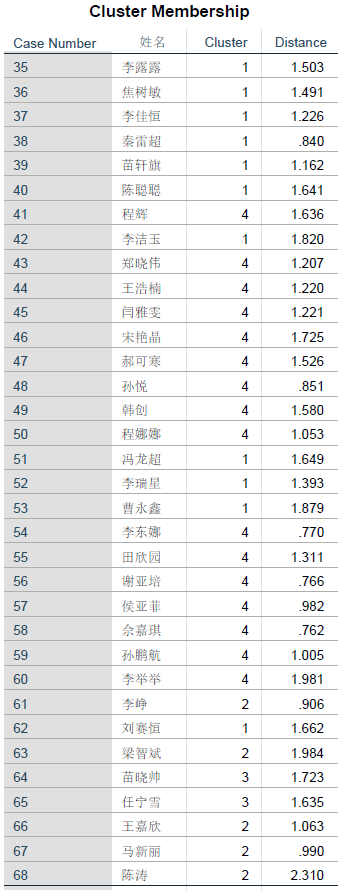
\includegraphics[scale=0.23]{聚类结果2.png}
        \end{minipage}
        \begin{minipage}{0.32\textwidth}
            \centering
            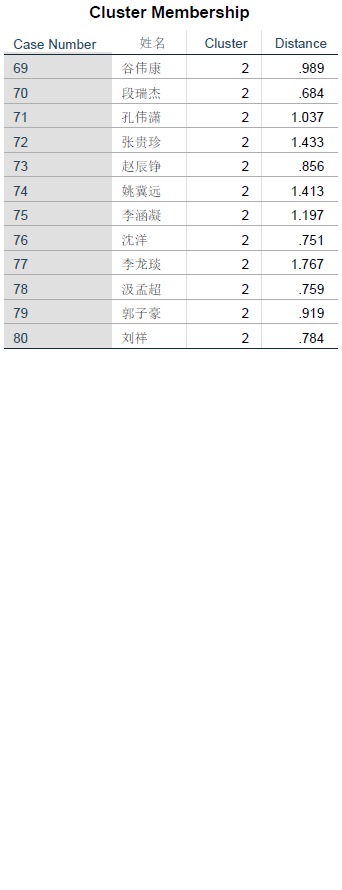
\includegraphics[scale=0.23]{聚类结果3.png}
        \end{minipage}
    \end{figure}
\end{frame}

\begin{frame}{各类中的样品数}
    \begin{center}
        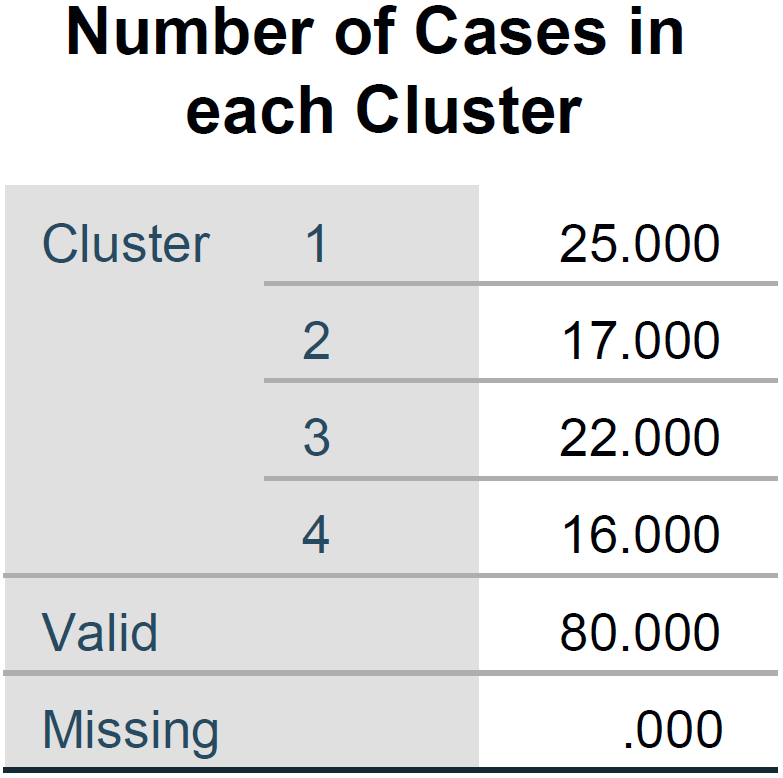
\includegraphics[scale=0.2]{各类的样品数.png}
    \end{center}
    \vspace{-0.5cm}
\end{frame}


\begin{frame}{方差分析表}
    \begin{center}
        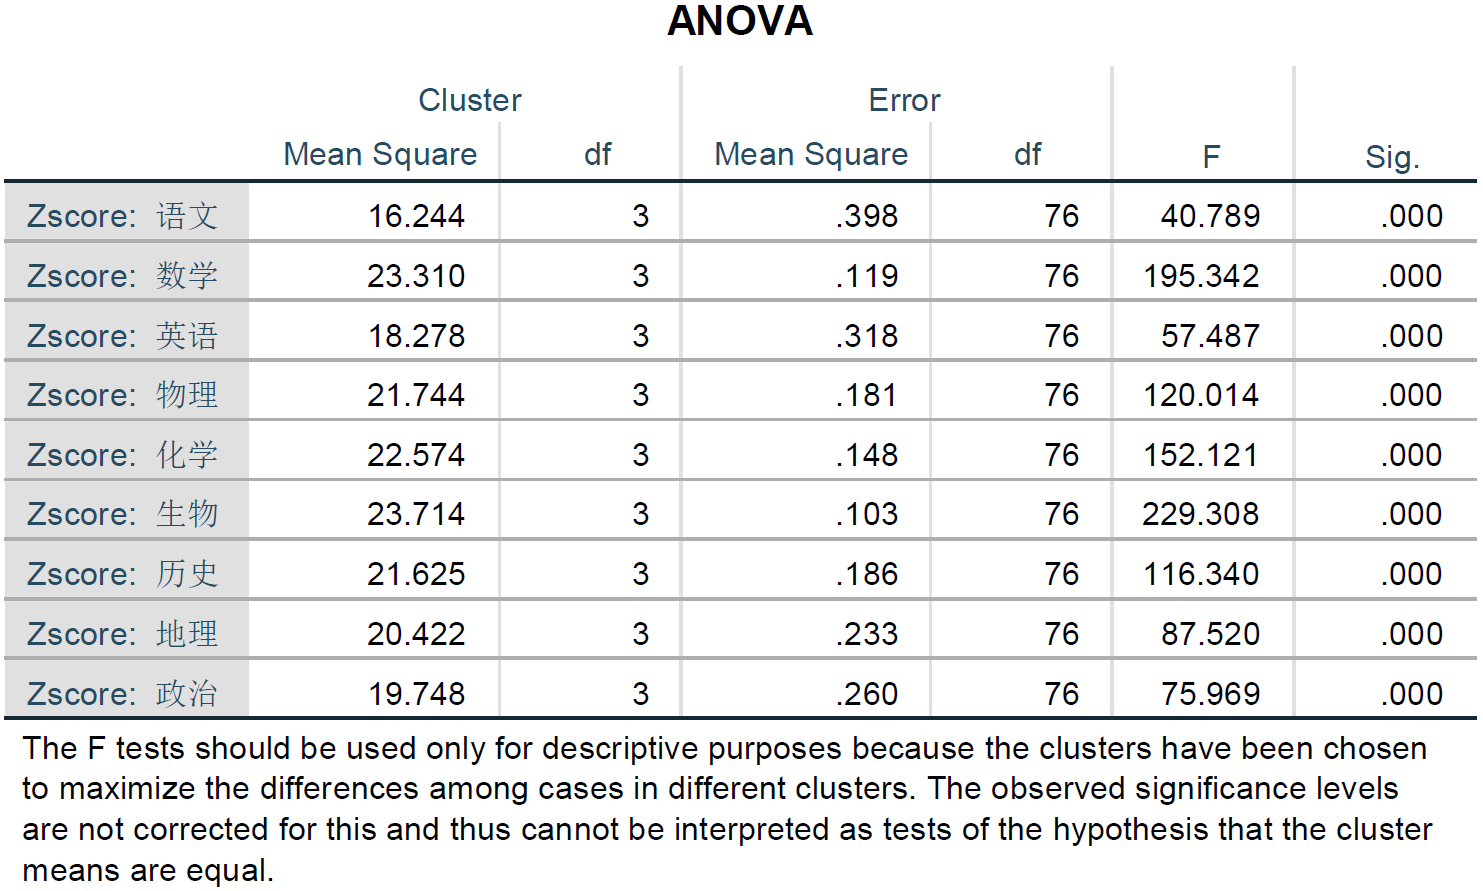
\includegraphics[scale=0.215]{方差分析表.png}
    \end{center}
    \vspace{-0.5cm}
\end{frame}
